\chapter{Results}
\label{chap:results}

\section{Method development}
\label{section:Results_Method_Development}
\subsection{Haemocyte medium: inhibition of aggregation}

\begin{figure}[!ht]
    \centering
    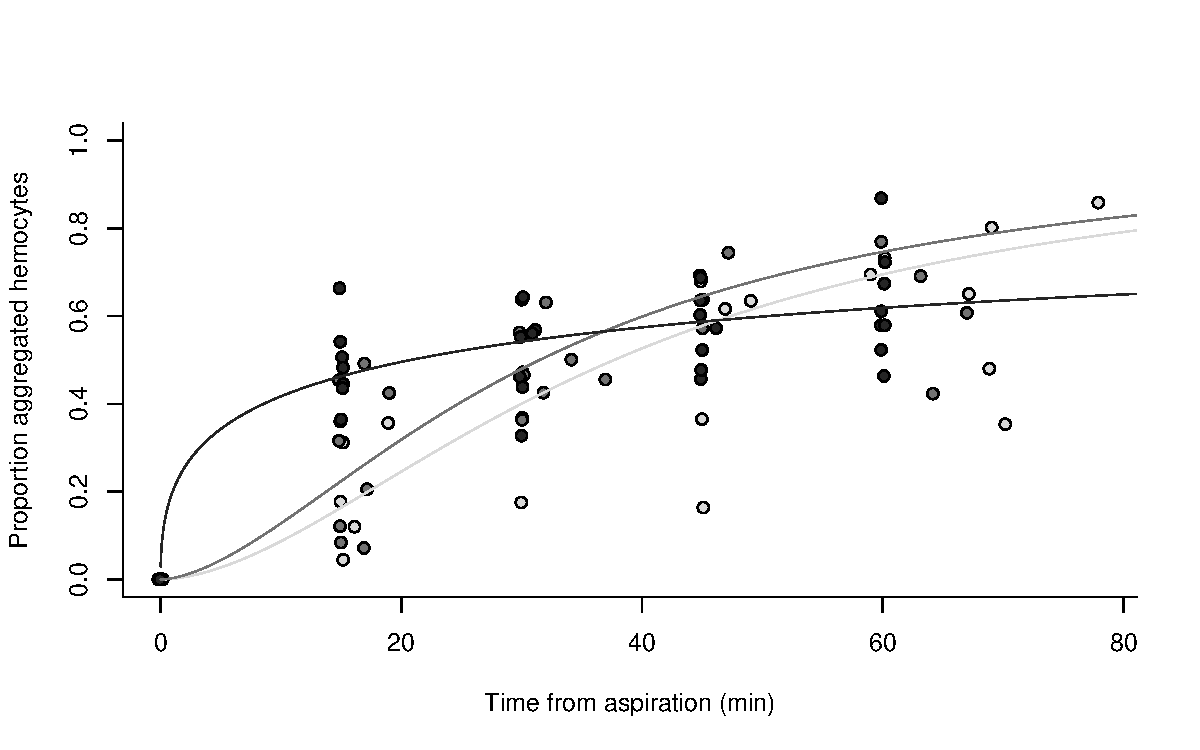
\includegraphics[width=1.0\textwidth]{figures/Method development/agg_plot_scaled.pdf}
    \caption{The proportion of aggregated hemocytes in 250 \micro L hemolymph withdrawn into an equal volume of Modified Alsever's Solution (\protect\lysegraacircle, n=7), Anticoagulant Buffer (\protect\graycircle, n=8) or Marine Physiological Saline Solution (\protect\darkgraycircle, n=8), plotted against time (min) after withdrawal from the posterior adductor muscle. The three regression lines illustrate the predicted proportions at time t for the three different buffers, as predicted by the fitted logistic regression model.}
    \label{fig:aggregation}
\end{figure}

Interpreting the logistic sub-models, it is evident that MAS and ACB effectively slowed the rate of aggregation during the first 30 minutes post-withdrawal. When MAS was used as hemocyte medium, the predicted mean proportion of aggregated hemocytes after 15 minutes was 0.16, 95\% CI [0.12, 0.22]. This was not significantly different from the predicted mean proportion when ACB was used (0.22, 95\% CI [0.18, 0.28]), but both buffers containing EDTA and lacking free Ca$^{2+}$ were predicted to have significantly lower hemocyte aggregation after 15 minutes, compared to samples that were withdrawn into MPSS and kept on ice (0.46, 95\% CI [0.33, 0.60]).

Although the model is over-dispersed, these estimates provided some insight into the three factor's relative abilities to prevent hemocyte aggregation within the first hour post-withdrawal. The combination of a Ca$^{2+}$-free and EDTA-containing buffer is effective in reducing hemocyte aggregation compared to simply diluting and keeping samples on ice. When using the latter method, visible aggregates were usually formed within the syringe immediately after hemolymph aspiration, even though the hemolymph saline has been pre-chilled at $\SI{4}{\celsius}$. For this method to be effective, the hemolymph most likely has to be diluted many-fold. Such an approach would be inconvenient when preparing microscopy slides of a certain desired cell density, and too time-consuming when acquiring 10.000 events on a flow cytometer. This methodology was therefore ruled out of question.

Comparing the relative effectiveness of MAS and ACB in preventing hemocyte aggregation, it is evident that neither citrate or maintaining a slightly acidic pH is required for the purpose. It might be that the slightly higher concentration of EDTA in ACB compensates for the lack of citrate. But either way, the acidic pH most likely plays a minor role. Since a high concentration of EDTA has been reported by some authors to impair hemocyte viability \cite{Grandiosa2018, Burkhard2009}, a further comparison of MAS and ACB with regards to acute effects on viability had to be investigated. [Include details in the function of glucose? Also short this down, because something is repeated.]

\subsection{Haemocyte medium: effect on viability}
 The percentage of necrotic hemocytes kept in at the three timepoints are presented in figure \ref{fig:BufferViability}. \lipsum[2]

\begin{figure}[!ht]
    \centering
    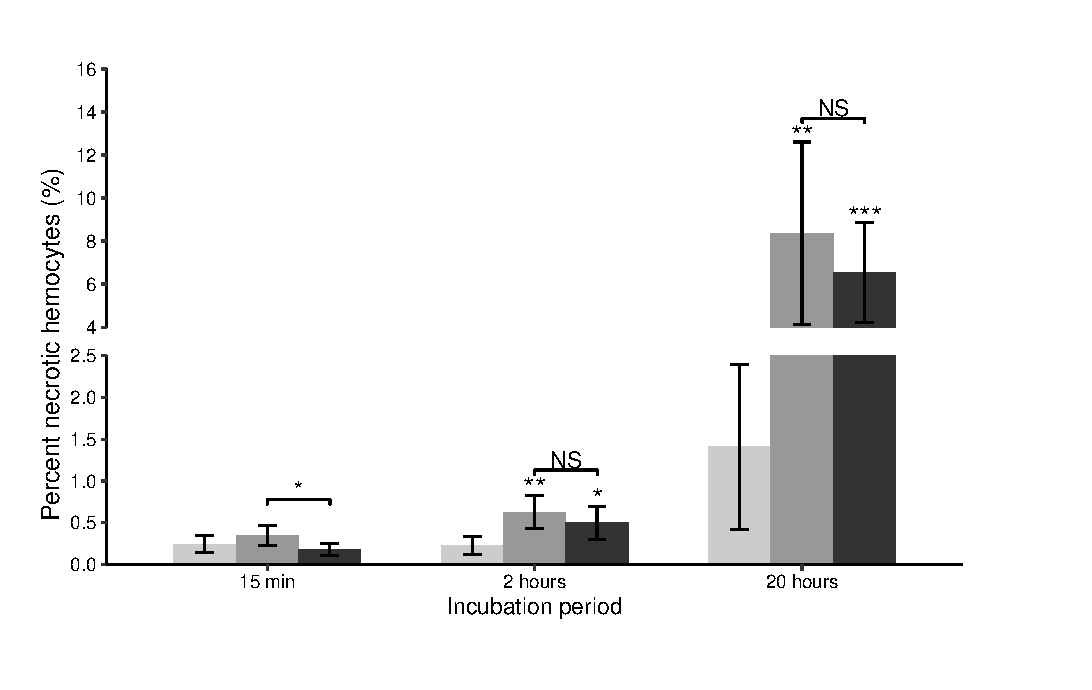
\includegraphics[width=1.13\textwidth]{figures/Method development/grouped bargraph scaled.pdf}
    \caption{The mean percentages of TO-PRO$^{TM}$-3 Iodide positive hemocytes after 15 minute, 2 hours and 20 hours incubation in \protect\lysegraabox \ Marine Physiological Saline Solution (n=8), \protect\customgraybox \ Anticoagulant Buffer (n=8) or \protect\darkgraybox \ Modified Alsever's Solution (n=8). Calcein acetoxymethyl (Invitrogen$^{TM}$) was used as a live cell counter-stain. Each datapoint is expressed as a percentage of 10.000 recorded hemocyte events, and the error bars represent 95\% confidence intervals of group means. Asterisks above error bars represent significance level of two sample t-test comparisons with }
    \label{fig:BufferViability}
\end{figure}

- Report results fro where I checked if EDTA changed the cytogram, because it would be nice to report that it doesn't affect them during the 15 minute incubation period.

\subsection{Cytologic characterization of \emph{M. edulis} hemocyte subpopulations}
The hemolymph of \emph{Mytilus edulis} comprised a mixed population of cells differing in size, granularity, morphometrics and Wright's-Giemsa staining profiles. If the haemocytes were allowed to spread prior to fixation and staining, the diversity further expanded as cells took on a variety of shapes and/or developed cytoplasmic extensions. From these morphological criteria, a total of three distinct cell types could be identified by light microscopy.

Based on the basophilic or eosinophilic nature of their granules and other cytoplasmic contents, cytologic staining with 3 \% Wright's-Giemsa or the Hemacolor\textsuperscript{\textregistered} kit gave rise to two distinct staining profiles: basophilic and eosinophilic haemocytes. The cytoplasm of eosinophilic hemocytes (Figure \ref{fig:celltypes}, K-O) were densely packed with pink to dark purple granules of varying size and abundance. Hence, they are referred to as eosinophilic granulocytes herein. Their individual granules were usually not distinguishable in a non-spread state, but instead gave their cytoplasm an irregular pink color (Figure \ref{fig:celltypes}, K and O). These haemocytes had cell diameters in the range of 6-16 \micro m, with a mean of 9.06$\pm1.25$ \micro m. Two strikingly homogeneous features of this cell type was a small acentrically located nucleus, and a regular spherical outline in a non-spread state. With abundant pink cytoplasm making up the majority of the cells' surface area - even in the smallest specimens - the eosinophilic granulocytes could also be characterized by a low nuclear-cytoplasmic ratio (N:C ratio). If not fixed and stained before smearing - or within minutes of applying haemolymph to a glass slide - eosinophilic granulocytes were almost exclusively observed as spread cells. 

\begin{figure}[!ht]
    \centering
    \includegraphics[width=1.0\textwidth]{figures/Anatomy/cell types brightfield updated 2.pdf}
    \caption{100$\times$ brightfield micrographs of the three haemocyte types found in the haemolymph of \emph{Mytilus edulis}, fixed and stained on glass slides with the Hemacolor\textsuperscript{\textregistered} kit before the hemocytes had time to spread notably. \textbf{(A-E)} Blast-like hyaline basophils. \textbf{(F-J)} Basophilic granulocytes. \textbf{(K-O)} Eosinophilic granulocytes. Samples were withdrawn into MPSS (1:1), scale bars = 10 \micro m.}
    \label{fig:celltypes}
\end{figure}

Compared to the eosinophilic granulocytes, the basophilic hemocytes encompassed a more heterogeneous population. Common to all of them were a larger nucleus that occupied more of the cells' total surface area (higher N:C ratio). The shape of which varied from spherical to oval, or had a distinct bean-shaped or irregular outline. But judged from the morphological criteria of cell size, granularity and N:C ratio, there were essentially two distinct subpopulations of basophilic haemocytes. One population of small hyaline blast-like haemocytes (5.63 $\pm{0.72}$ \micro m) displaying only a marginal rim of dove blue cytoplasm and no apparent cytoplasmic granules (Figure \ref{fig:celltypes}, A-E), and one population of larger haemocytes (8.07 $\pm{1.25}$ \micro m), displaying abundant basophilic cytoplasm with varying degrees of cytoplasmic granulation and vacuolation (Figure \ref{fig:celltypes}, F-J). The basophillic granules appeared much smaller than those of the eosinophilic granulocytes, and were usually not very conspicuous unless haemocytes were subjected to osmotic swelling prior to fixation and staining. Under differential interference contrast (DIC) illumination however, their granules created highly irregular surface topographies in spread cells that could be observed without such treatment. On the basis of these morphological differences, the basophilic haemocytes were subdivided into blast-like haemocytes and basophilic granulocytes herein. 

\begin{figure}[!ht]
    \centering
    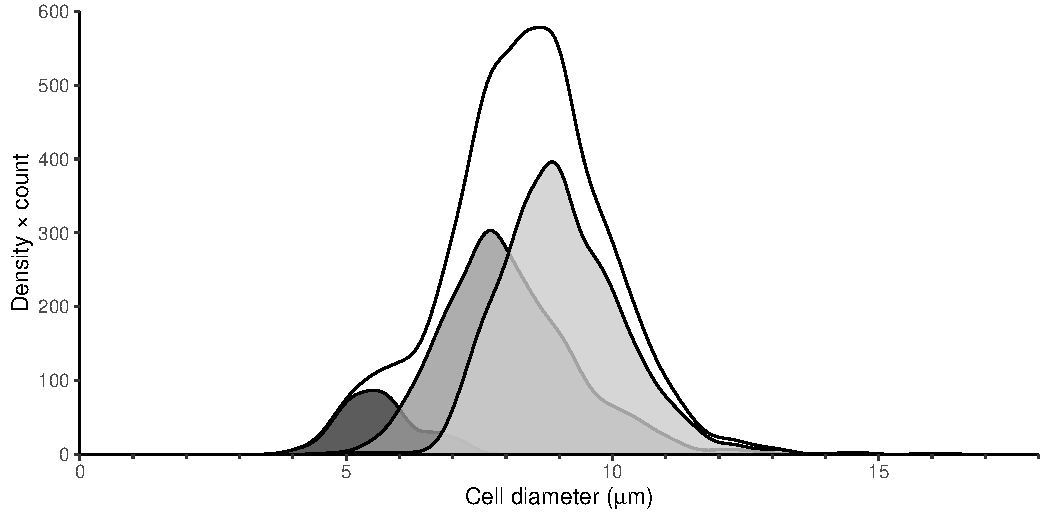
\includegraphics[width=1.0\textwidth]{figures/Anatomy/diameters scaled density plot.pdf}
    \caption{Size distribution of \protect\dimgraybox \ small blast-like basophils (n=154), \protect\lightgraybox \ basophilic granulocytes (n=821), \protect\lysegraabox \ eosinophilic granulocytes (n=1030) and \protect\whitebox \ the total haemocyte population of \emph{Mytilus edulis} (n=2005). The diameters of 100 formaldehyde-fixed haemocytes was measured in each of 20 individual mussels, and the density was scaled to the number of observations of each cell type.}
    \label{fig:Diameters}
\end{figure}

The size distributions of the three haemocyte types are shown as three kernel-smoothened density plots in Figure \ref{fig:Diameters}, together with that of the total haemocyte population. The densities have been scaled to the number of observations of each cell type, such that their relative proportions can be visualized. In the 20 adult mussels examined here, the small blast-like basophils were the least abundant cell type, making up 7.9 $\pm{5.6}$ \% of the total haemocyte population. In 14 out of 20 mussels, the blast-like basophils were followed by the basophilic granulocytes, with a mean relative proportion of 40.7 $\pm{12.9}$ \%. In spite of constituting similar proportions as the basophilic granulocytes in several mussels, the eosinophilic granulocytes were the most abundant cell type in the haemolymph of \emph{M. edulis}, constituting 51.5 $\pm{15.3}$ \% of the total haemocyte population, on average. The relative proportions of basophilic and eosinophilic granulocytes did however vary to a large extent between individual mussels, as reflected by their standard deviations. [Should I include t.tests in this section? - note: unequal sample sizes]

When incorporating the Coulter Counter data in this section, this article can be used to reference the accuracy of the electronic cell size method which it uses: Mattern CFT, Brackett FS, Olson BJ. Determination of number and size of particles by electrical gating: blood cells. J Appl Physiol 1957;10:56–70


\subsection{Flow cytometric characterization of haemocyte subpopulations by light-scatter measurements}
With the BD Accuri C6 Plus benchtop flow cytometer, a maximum of three distinct hemocyte subpopulations (clusters) could be distinguished from \emph{M. edulis} hemolymph on Forwards scatter (FCS) vs. Side scatter (SSC) dotplots. These subpopulations correspond to clusters 1, 2 and 3 . Falling within the singlet gate in Figure \ref{fig:fsc_vs_ssc}, shown with SSC on both linear and logarithmic scales. The events in cluster 1 exhibit low FSC- and SSC-values relative to cluster 2 and 3, suggesting that it is populated by small and uncomplex cells. Events in both clusters 2 and 3 display higher FSC-values, but are often partially separated according to SSC.  and cluster 3 have more cells of very large diameter. is made up of cells with medium SSC- and FSC-values, with a few events having high those in gate 2 exhibit medium FSC- and SSC-values, including some events with high FSC-values, while the cells in gate 3 have high SSC-values with most of the cells

\begin{figure}[!ht]
    \centering
    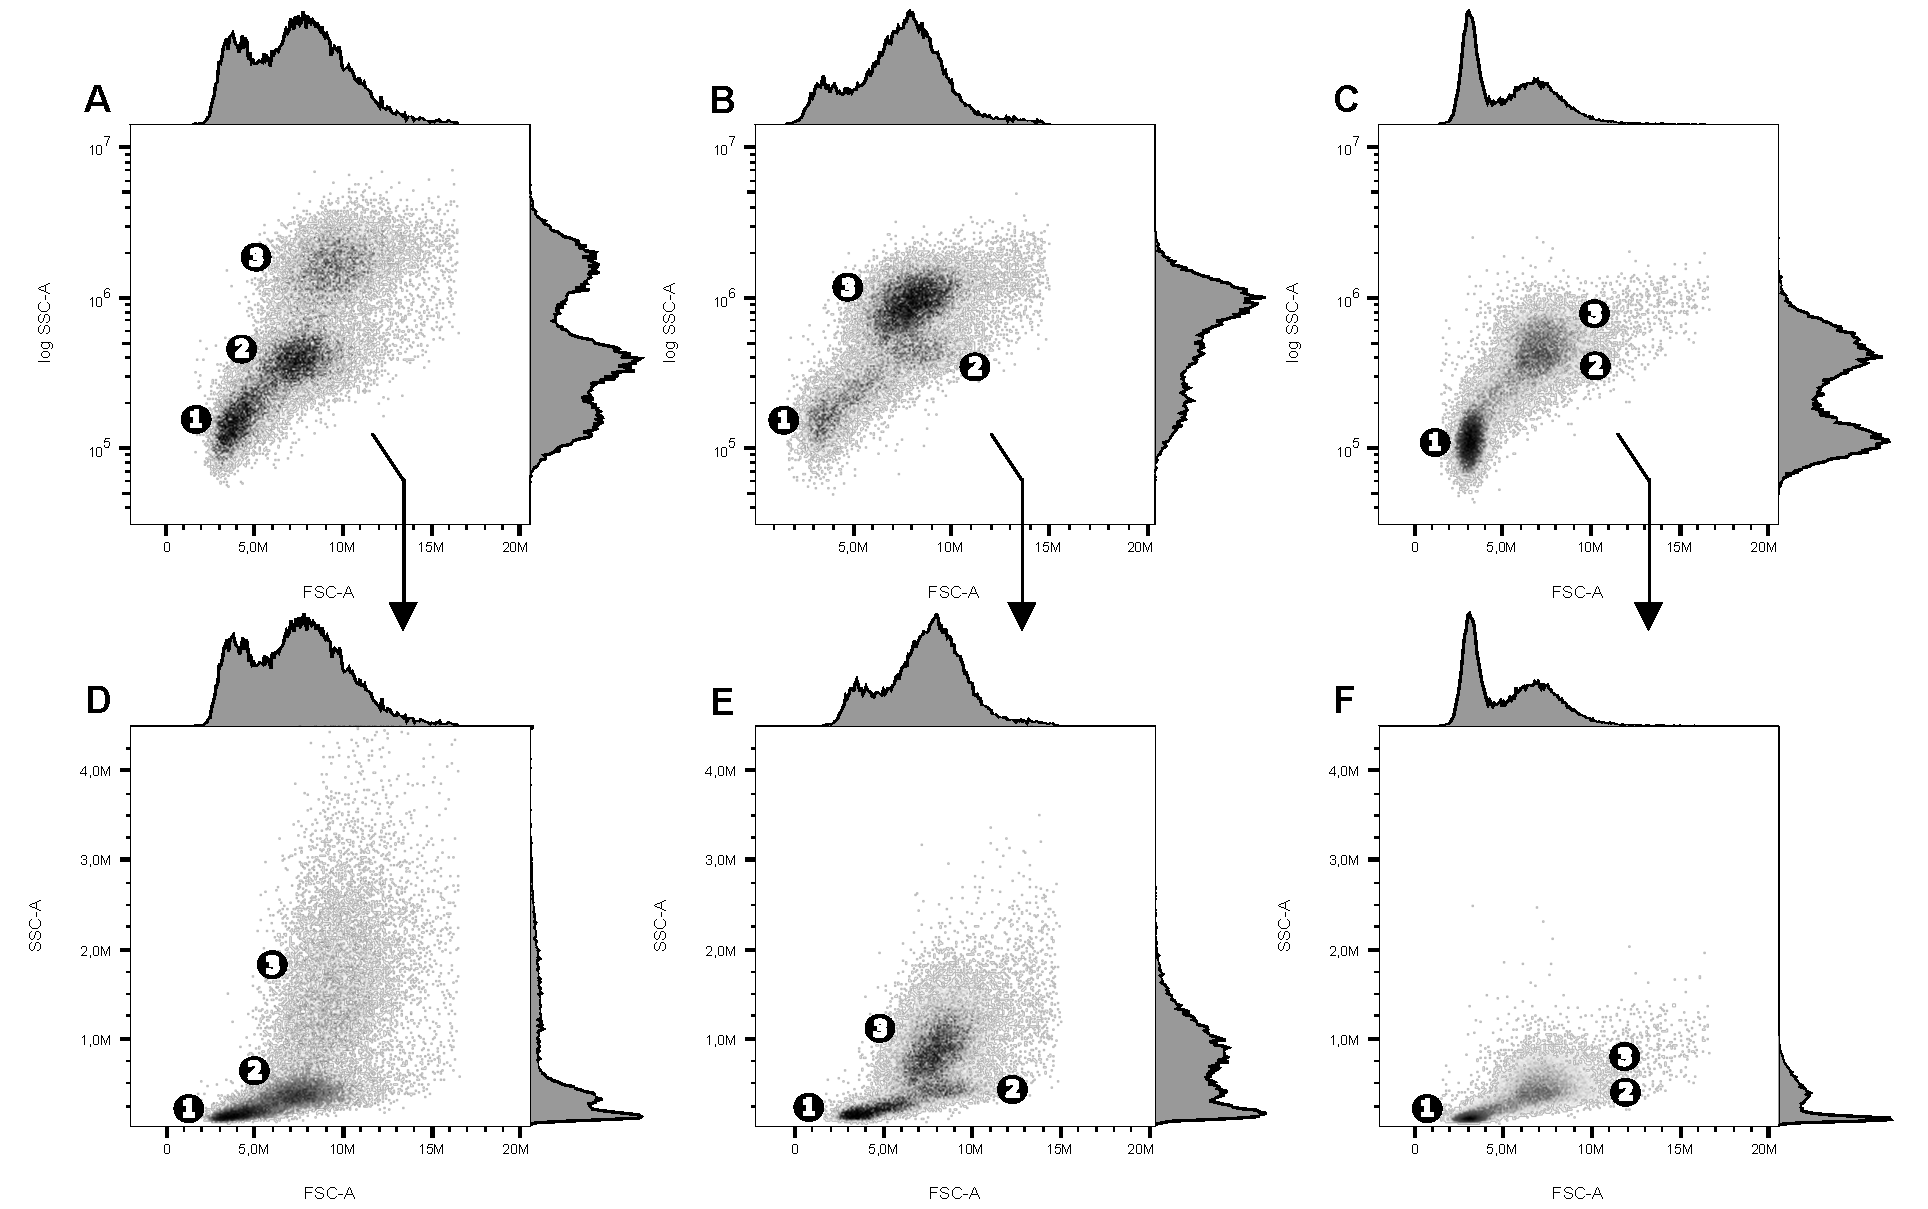
\includegraphics[width=1.0\textwidth]{figures/Gating strategy/scatter profiles 30k with let num.pdf}
    \caption{Hemocyte subpopulations distinguishable according to FSC vs. SSC \textbf{A} Bla bla bla.. Mention that the actual proportion was calculated counting 1000 hemocytes, and that the gates were adjusted to the true value.}
    \label{fig:fsc_vs_ssc}
\end{figure}

and are most likely corresponding to the small agranular cells shown in Figure [ref to Figure with cell morphology and Giemsa staining profile], with a large oval nucleus and a thin rim of basophilic staining cytoplasm. Herein we will refer to them as agranular basophils according to their Giemsa staining profile. Because of their smaller size relative to the cells in cluster 2 and 3; they are readily distinguishable with a separate peak in Coulter Counter particle-size distributions, and have cell diameters between 5.5-8 \micro m [include Figure].

In some adult mussels, however, the basophilic and eosinophilic granulocyte subpopulations are partly overlapping with regard to internal complexity, i.e., SSC. Since the BD Accuri C6 Plus isn't equipped with adjustable laser gain settings, these subpopulations could not be separated further instrumentally. Thus, any attempts to gate on these subpopulations based solely on light scattering profiles, would in some mussels introduce considerable uncertainty into their relative proportions. [Find the proportion of mussels where they are not well separated, and report that number instead of saying "some" mussels here.]


\subsection{Relating the cytologically defined cell types to light-scatter profiles}
Hemocyte subpopulations and clusters. Light-scattering properties (optical characteristics).
The first round of Percoll separation yielded 96.1 \% eosinophilic granulocytes in the 43/90\% fraction.
The second round of percoll gradient separation yielded: 15\%-33\% interface: FCM = 97\% basophils, microscopy = 96.14 \% basophils (7.72\% blast-like and 88.42\%) (= 3.86 \% eosinophils) 43\%-90\% interface: FCM = 94\%, microscopy = 97.52 \%.

\begin{figure}[!ht]
    \centering
    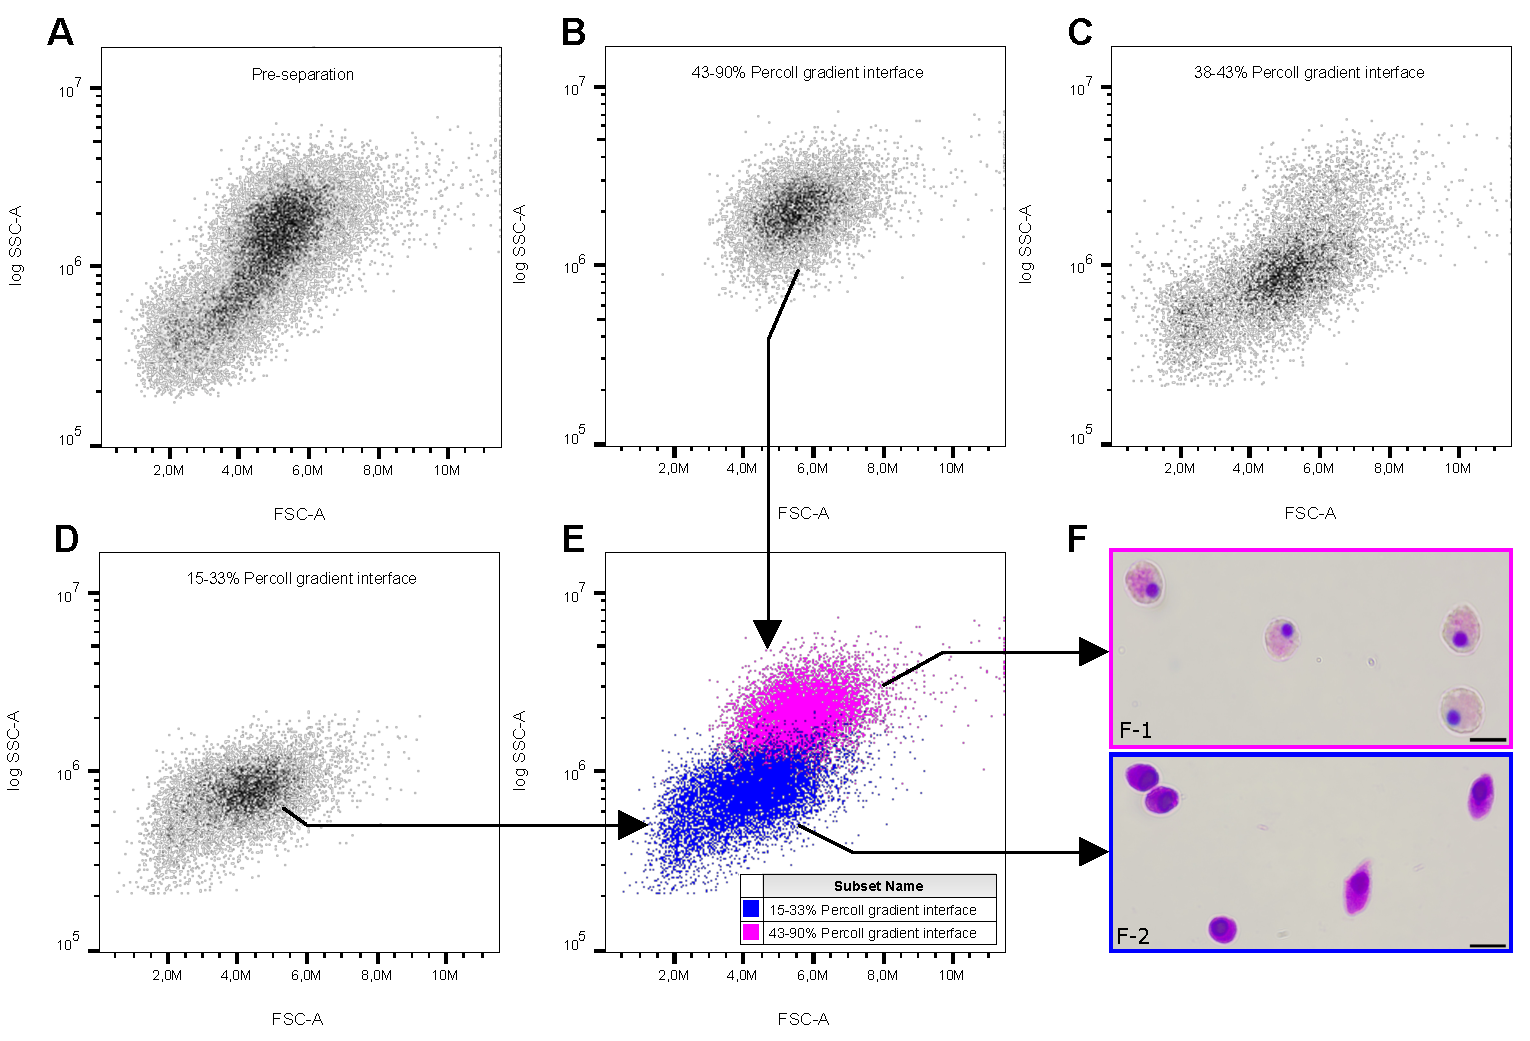
\includegraphics[width=1.0\textwidth]{figures/Method development/PERCOLL SEP II final.pdf}
    \caption{\textbf{Confirmation of the light scattering profiles of eosinophilic and basophilic granulocytes pre-separated by discontinuous density centrifugation. A} Light scattering profile of the 95\% pure eosinophilic fraction that separated out on top of the 43-90\% Percoll gradient interface. \textbf{B} Bla bla bla eosin separation bla bla...}
    \label{fig:Percoll-dotplots}
\end{figure}



\begin{figure}[!ht]
    \centering
    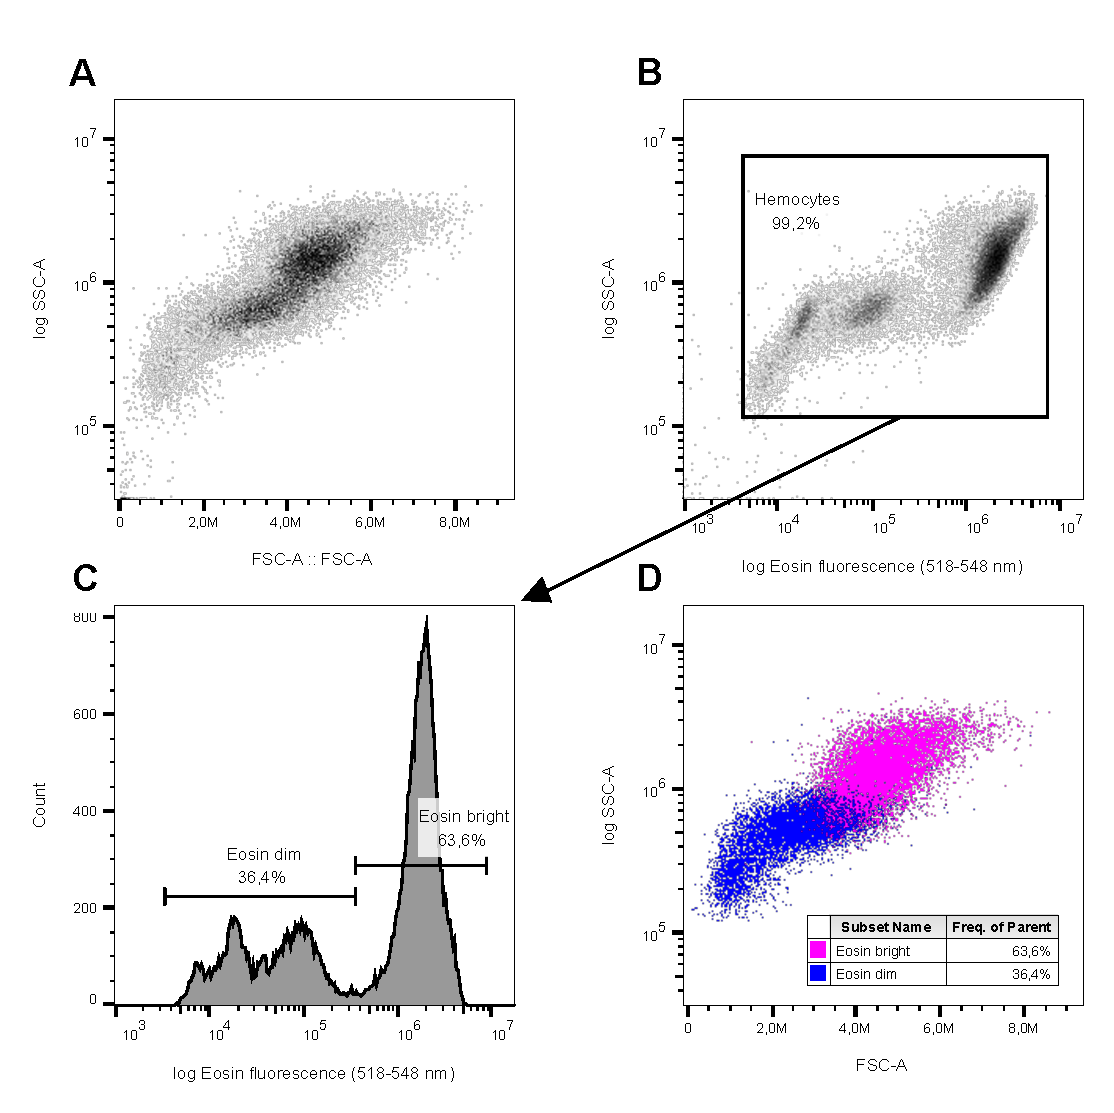
\includegraphics[width=1.0\textwidth]{figures/Method development/Eosin exp figure for LaTeX.pdf}
    \caption{\textbf{Identification eosinophilic granulocytes. A)} Representative light scatter profiles of... \textbf{B)} }
    \label{fig:eosin_exp2}
\end{figure}

[After the eosinophils had sedimented in the MAS buffer (sample M2 in sedimentation dataset) for 2 hours post-withdrawal (1:1), the percentage of eosinophils remaining in suspension were 72/1075 = 6.6976 \%. The 10k ToPro3 Calcein stained plot shows 7.91\%.]
\newpage



\subsection{Scoring of necrotic haemocytes by flow cytometry}
\subsubsection{Determination of optimal TO-PRO$^{TM}$-3 Iodide staining concentration}
Viable and \ce{MeOH}-killed haemocytes could be separated according to TO-PRO-3 Iodide fluorescence when incubated in concentrations $\geq$ 100 nM (Fig. \ref{fig:ToPro3_stain_opt}A). As seen in Fig. \ref{fig:ToPro3_stain_opt}B, the resolution between ToPro3$^{-}$ and ToPro3$^{+}$ events drastically increased in the range of 100 nM to 2 \micro M TO-PRO$^{TM}$-3 Iodide, with a linear decrease when incubated in concentrations > 2 \micro M. The decreasing difference in mean fluorescent intensity (MFI) > 2 \micro M reflects both a saturation of dsDNA-bound TO-PRO-3



\begin{figure}[h]
    \centering
    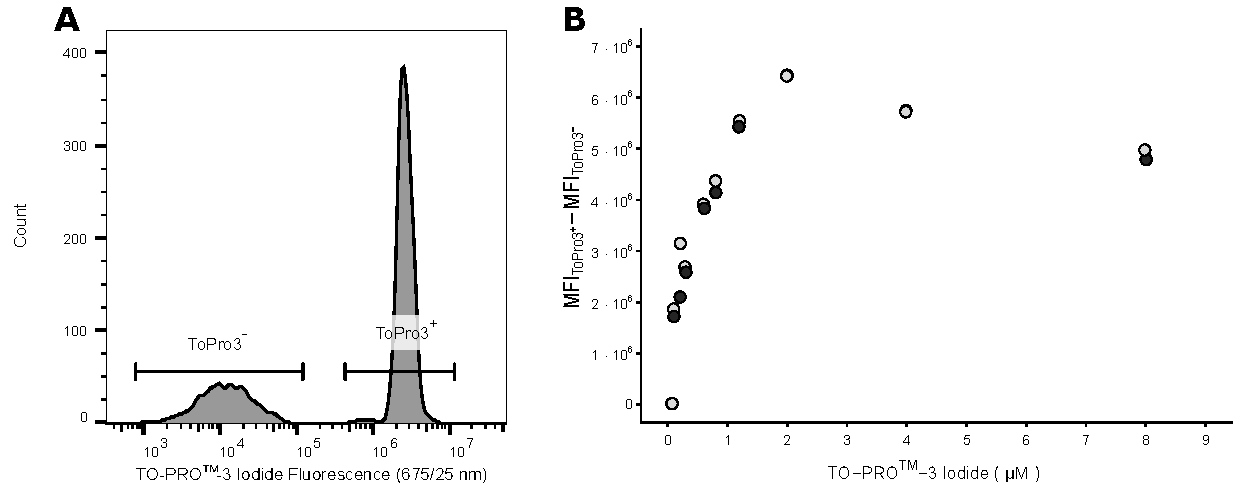
\includegraphics[width=1.0\textwidth]{figures/Method development/ToPro3 stainopt figure mean.pdf}
    \caption{\textbf{Experimental determination of the optimal TO-PRO$^{TM}$-3 Iodide concentration for a dye exclusion test of membrane integrity}. 10 aliquots of pooled methanol-killed (70\% \ce{MeOH}, 30 min) and viable haemocytes (1:1) were stained with different concentrations of TO-PRO$^{TM}$-3 Iodide (30 nM - 8 \micro M). 640 nm-exited fluorescence from dsDNA-bound TO-PRO$^{TM}$-3 Iodide were collected on the FL4 detector (675/25 nm) of the BD Accuri C6 Plus flow cytometer, recording 10.000 events from each sample after 15 and 30 minute incubation. \textbf{A)} ToPro3$^{-}$ and ToPro3$^{+}$ events were gated on log scale for each sample, \textbf{B)} and their difference in mean fluorescent intensity (MFI) after 15 (\protect\lysegraacircle) and 30 minutes (\protect\darkgraycircle) of incubation were plotted against the concentration of TO-PRO$^{TM}$-3 Iodide.}
    \label{fig:ToPro3_stain_opt}
\end{figure}
































\newpage
\section{Hybrid FCM/Microscopy MN Cytome Assay: Results}
\subsection{MN and other nuclear anomalies}
\subsection{Haemocyte viability: membrane integrity}
\subsection{Apoptosis assay}
\subsection{Haemocyte differential counts and concentration}

